% This is "sig-alternate.tex" V2.0 May 2012
% This file should be compiled with V2.5 of "sig-alternate.cls" May 2012
%
% This example file demonstrates the use of the 'sig-alternate.cls'
% V2.5 LaTeX2e document class file. It is for those submitting
% articles to ACM Conference Proceedings WHO DO NOT WISH TO
% STRICTLY ADHERE TO THE SIGS (PUBS-BOARD-ENDORSED) STYLE.
% The 'sig-alternate.cls' file will produce a similar-looking,
% albeit, 'tighter' paper resulting in, invariably, fewer pages.
%
% ----------------------------------------------------------------------------------------------------------------
% This .tex file (and associated .cls V2.5) produces:
%       1) The Permission Statement
%       2) The Conference (location) Info information
%       3) The Copyright Line with ACM data
%       4) NO page numbers
%
% as against the acm_proc_article-sp.cls file which
% DOES NOT produce 1) thru' 3) above.
%
% Using 'sig-alternate.cls' you have control, however, from within
% the source .tex file, over both the CopyrightYear
% (defaulted to 200X) and the ACM Copyright Data
% (defaulted to X-XXXXX-XX-X/XX/XX).
% e.g.
% \CopyrightYear{2007} will cause 2007 to appear in the copyright line.
% \crdata{0-12345-67-8/90/12} will cause 0-12345-67-8/90/12 to appear in the copyright line.
%
% ---------------------------------------------------------------------------------------------------------------
% This .tex source is an example which *does* use
% the .bib file (from which the .bbl file % is produced).
% REMEMBER HOWEVER: After having produced the .bbl file,
% and prior to final submission, you *NEED* to 'insert'
% your .bbl file into your source .tex file so as to provide
% ONE 'self-contained' source file.
%
% ================= IF YOU HAVE QUESTIONS =======================
% Questions regarding the SIGS styles, SIGS policies and
% procedures, Conferences etc. should be sent to
% Adrienne Griscti (griscti@acm.org)
%
% Technical questions _only_ to
% Gerald Murray (murray@hq.acm.org)
% ===============================================================
%
% For tracking purposes - this is V2.0 - May 2012

\documentclass{sig-alternate}

\usepackage{url}

\begin{document}
%
% --- Author Metadata here ---
\conferenceinfo{Social Machines Workshop}{2013, Paris, France}
%\CopyrightYear{2007} % Allows default copyright year (20XX) to be over-ridden - IF NEED BE.
%\crdata{0-12345-67-8/90/01}  % Allows default copyright data (0-89791-88-6/97/05) to be over-ridden - IF NEED BE.
% --- End of Author Metadata ---

\title{A Framework for Classification of Social Machines}
%\subtitle{[Extended Abstract]
%\titlenote{A full version of this paper is available as
%\textit{Author's Guide to Preparing ACM SIG Proceedings Using
%\LaTeX$2_\epsilon$\ and BibTeX} at
%\texttt{www.acm.org/eaddress.htm}}}
%
% You need the command \numberofauthors to handle the 'placement
% and alignment' of the authors beneath the title.
%
% For aesthetic reasons, we recommend 'three authors at a time'
% i.e. three 'name/affiliation blocks' be placed beneath the title.
%
% NOTE: You are NOT restricted in how many 'rows' of
% "name/affiliations" may appear. We just ask that you restrict
% the number of 'columns' to three.
%
% Because of the available 'opening page real-estate'
% we ask you to refrain from putting more than six authors
% (two rows with three columns) beneath the article title.
% More than six makes the first-page appear very cluttered indeed.
%
% Use the \alignauthor commands to handle the names
% and affiliations for an 'aesthetic maximum' of six authors.
% Add names, affiliations, addresses for
% the seventh etc. author(s) as the argument for the
% \additionalauthors command.
% These 'additional authors' will be output/set for you
% without further effort on your part as the last section in
% the body of your article BEFORE References or any Appendices.

\numberofauthors{1} %  in this sample file, there are a *total*
% of EIGHT authors. SIX appear on the 'first-page' (for formatting
% reasons) and the remaining two appear in the \additionalauthors section.
%
\author{
% You can go ahead and credit any number of authors here,
% e.g. one 'row of three' or two rows (consisting of one row of three
% and a second row of one, two or three).
%
% The command \alignauthor (no curly braces needed) should
% precede each author name, affiliation/snail-mail address and
% e-mail address. Additionally, tag each line of
% affiliation/address with \affaddr, and tag the
% e-mail address with \email.
%
% 1st. author
\alignauthor
Authors\\
       \affaddr{Web and Internet Science Group}\\
       \affaddr{University of Southampton}\\
       \affaddr{Southampton, UK}\\
       \email{\{a,b,c,d,wh,nrs\}@ecs.soton.ac.uk}
}
% There's nothing stopping you putting the seventh, eighth, etc.
% author on the opening page (as the 'third row') but we ask,
% for aesthetic reasons that you place these 'additional authors'
% in the \additional authors block, viz.
%\additionalauthors{Additional authors: John Smith (The Th{\o}rv{\"a}ld Group,
%email: {\texttt{jsmith@affiliation.org}}) and Julius P.~Kumquat
%(The Kumquat Consortium, email: {\texttt{jpkumquat@consortium.net}}).}
%\date{30 July 1999}
% Just remember to make sure that the TOTAL number of authors
% is the number that will appear on the first page PLUS the
% number that will appear in the \additionalauthors section.

\maketitle
\begin{abstract}

This paper provides a framework for...

\end{abstract}

% A category with the (minimum) three required fields
%\category{H.4}{Information Systems Applications}{Miscellaneous}
%A category including the fourth, optional field follows...
%\category{D.2.8}{Software Engineering}{Metrics}[complexity measures, performance measures]

%\terms{Theory}

%\keywords{ACM proceedings, \LaTeX, text tagging}

\section{Introduction (0.5 page)}

What are social machines and why are they important

An emerging, interdisciplinary field of research and development with a growing number of social machine instances and studies about them

We propose a classification framework for social machines. Targeted audiences

* research community: shared terminology, set of key features and their possible instantiations based on the analysis of a relevant set of 50 (?) social machines (both popular systems as well as long tail systems); facilitates the study of design and evolution patterns; supports research on how communities emerge and develop and organizational studies (mechanism design, incentives); different research approaches can be better compared and aligned.

* developer community: provides a theoretical grounding for the realization of new systems, informs system design and operation (what features should be implemented, what features are more important than others); enables predictions on user behavior and community development.

The framework is based on interviews with XXX researchers covering XXX systems and was preliminary evaluated with respect to ...


\section{Methodology (1 page)}

How was the classification framework defined

* interviews with XXX researchers on key descriptive features of systems they are familiar with

* consolidation of features listed for a resulting set of 50 (?) social machines

* grid analysis to identify groups of similar systems

* evaluation with respect to correctness, completeness, clarity, extendability in user survey, additional data set of XXX systems


\section{Classification framework (2 pages)}

First explain main principles: Distinction between application system and enabling technology; contributions, actions, activities, purpose, etc

\subsection{The Hierarchy/Polyarchical relationship of social machines}

While determining a set of social machines, one clear distinction was between social machine frameworks, such as MediaWiki and Ushahidi, which enable
social machines to be created, and instantiations of those frameworks into social machines that have been created for a specific purpose, such as Wikipedia
and Ushahidi Haiti. However, through further investigation, we discovered that the distinction between framework and instantiations was not the only
differentiator. Specifically, that some social machines could also have sub-machines or communities within them, that are working to solve different problems,
within the context of the larger machine. For example, Wikipedia is an instantiation of the MediaWiki framework, but there are a large number of
communities within Wikipedia that work on domain-specific areas, such as those contributing in areas of science and technology\footnote{Visualisation of Wikipedia Science Communities: \url{http://www.olihb.com/WikiCommunities/}}. However, we must also note that wikipedia is primarily split into communities of language, with the English, German and French wikipedias having the largest number of articles. It is therefore possible to analyse wikipedia into a hierarchy, from MediaWiki, to the languages of Wikipedia, down to the domain-specific communities. We explored this idea further, to include other social machines, and links where social machines utilise other social machines in order to function. For example, the social machine used by the Obama '12 US Presidential campaign~\cite{obamakieron}, which relied on social machines such as Twitter and Facebook. A resulting polyarchy is shown in Figure \ref{polyarchy}, which classifies levels as Infrastructure, Frameworks, Services and Causes/Groups.

\begin{figure*}[htb]
\begin{center}
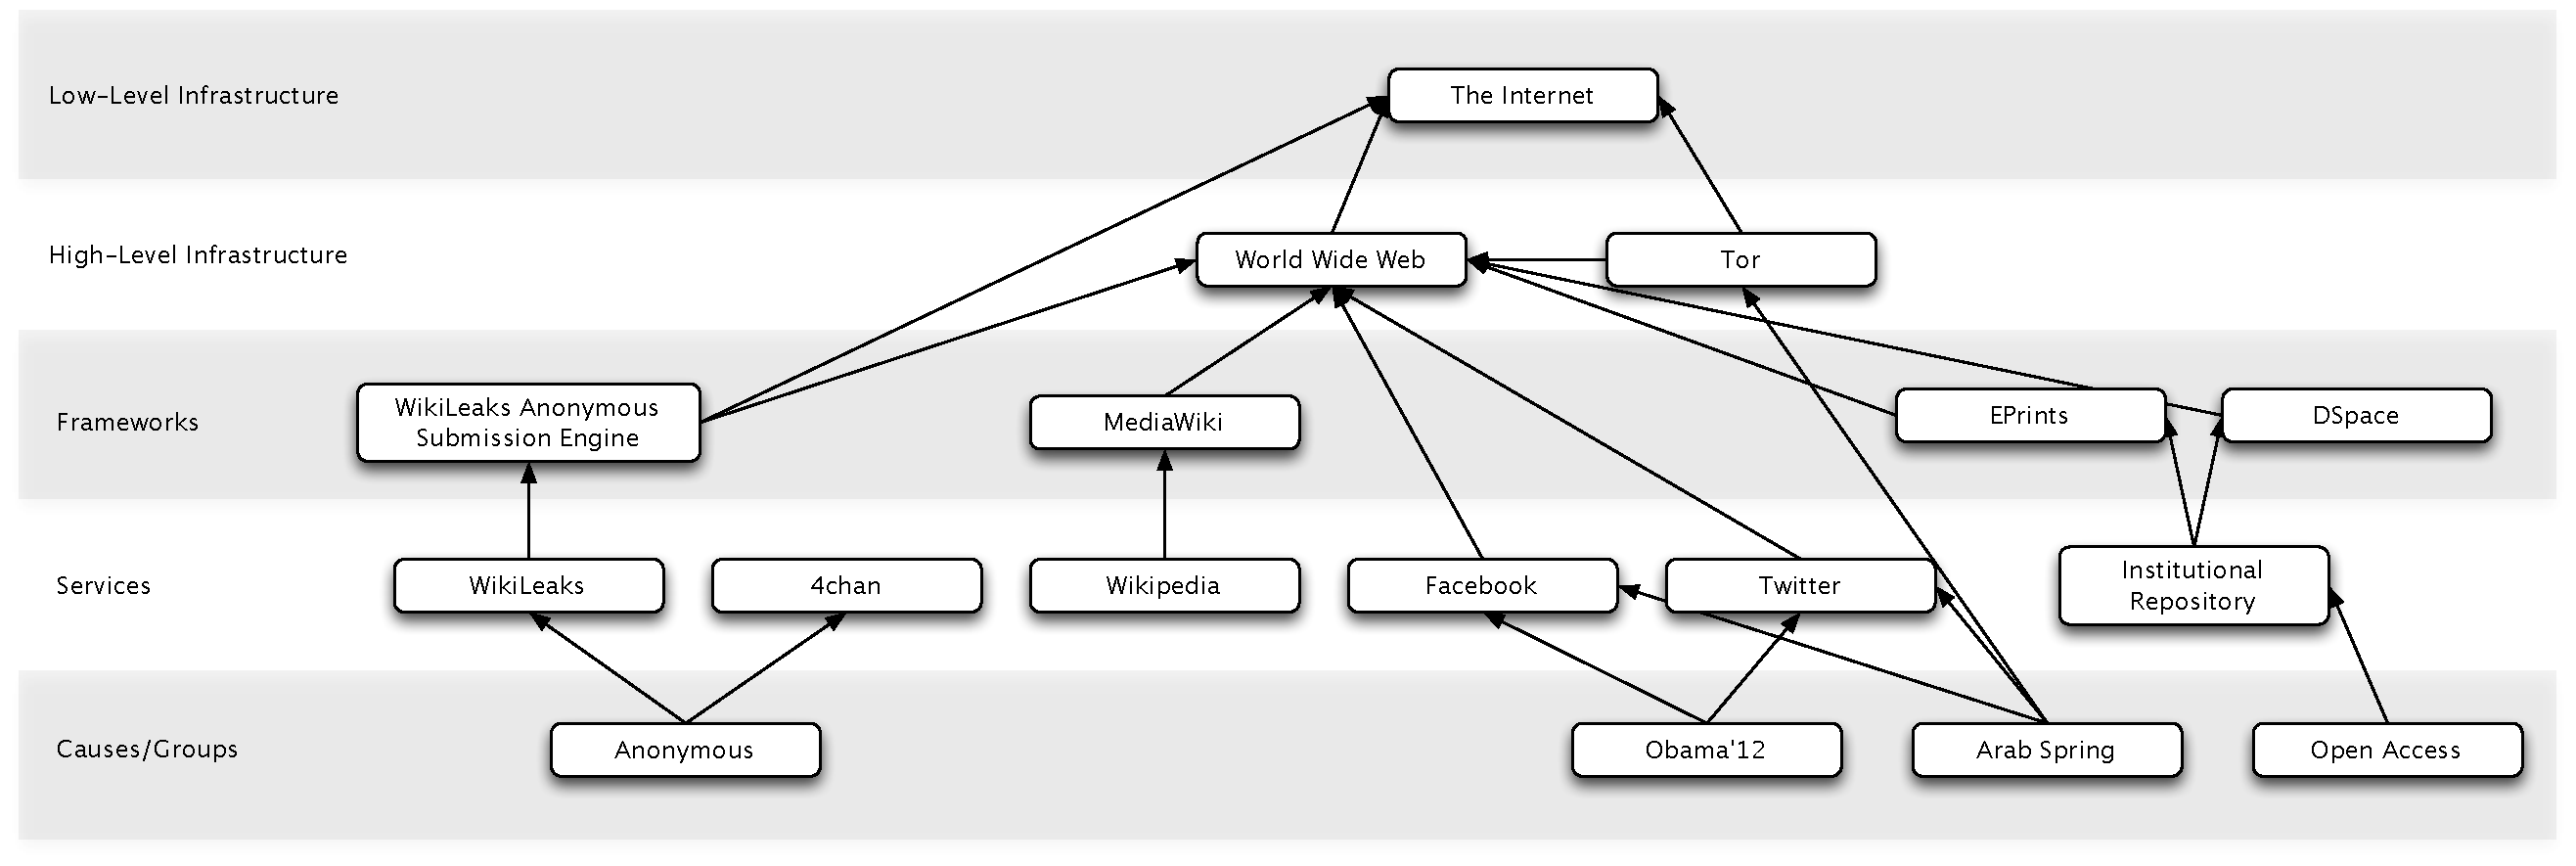
\includegraphics[width=18cm]{img/polyarchy.pdf}
\caption{A polyarchy of Social Machines, illustrating the infrastructure and frameworks used by social machines, and machine-machine usage.} \label{polyarchy}
\end{center}
\end{figure*}

\subsection{Artefacts of Social Machines}

Our next observation was that there are a number of shared artefact types that can be classified within the context of social machines. Specifically that
there are ``intentions'' that motivate the use of social machines, ``actions'' that are directly performed by participants of social machines, and ``contributions``
that result from the use of social machines. We have taken these abstract concepts, and mapped them to a number of well-known social machines in order
to demonstrate that these concepts can be used to compare and contrast different machines.





\section{Usage examples (0.5 page)}
Wikipedia

GalaxyZoo (?)

Ushahidi

Facebook

MechanicalTurk

GWAPs


\section{Related work (0.5 pages)}

existing classification systems in CSCW, collective intelligence, social computing systems

\section{Conclusions and future work (0.5 pages)}

Detail evaluation plans

Feedback from different disciplines, and from the developers community

%ACKNOWLEDGMENTS are optional
\section{Acknowledgments}

This work is supported under SOCIAM: The Theory and Practice of Social Machines.  The SOCIAM Project is funded by the UK Engineering and Physical Sciences Research Council (EPSRC) under grant number EP/J017728/1 and comprises the Universities of Southampton, Oxford and Edinburgh.

%
% The following two commands are all you need in the
% initial runs of your .tex file to
% produce the bibliography for the citations in your paper.
\bibliographystyle{abbrv}
\bibliography{sigproc}  % sigproc.bib is the name of the Bibliography in this case
% You must have a proper ".bib" file
%  and remember to run:
% latex bibtex latex latex
% to resolve all references
%
% ACM needs 'a single self-contained file'!
%
%APPENDICES are optional


\balancecolumns % GM June 2007
% That's all folks!
\end{document}
